\documentclass[a4paper,12pt]{scrartcl}

%code block package
\usepackage{listings}
\usepackage{graphicx}
\usepackage[utf8]{inputenc}
\usepackage[english]{babel}
\usepackage{geometry}
\usepackage{multicol}
\geometry{hmargin=2cm,vmargin=2cm}
\usepackage{hyperref}
\hypersetup{
    colorlinks,
    citecolor=black,
    filecolor=black,
    linkcolor=black,
    urlcolor=black
}

% -- Defining colors:
\usepackage[dvipsnames]{xcolor}
\definecolor{codegreen}{rgb}{0,0.6,0}
\definecolor{codegray}{rgb}{0.5,0.5,0.5}
\definecolor{codepurple}{rgb}{0.58,0,0.82}
\definecolor{backcolour}{rgb}{0.95,0.95,0.92}% Definig a custom style:
\lstdefinestyle{mystyle}{
    backgroundcolor=\color{backcolour},   
    commentstyle=\color{codepurple},
    keywordstyle=\color{orange},
    numberstyle=\tiny\color{codegray},
    stringstyle=\color{codepurple },
    basicstyle=\ttfamily\footnotesize\bfseries,
    breakatwhitespace=false,         
    breaklines=true,                 
    captionpos=t,                    
    keepspaces=gal,                 
    numbers=left,                    
    numbersep=5pt,                  
    showspaces=false,                
    showstringspaces=false,
    showtabs=false,                  
    tabsize=2
}% -- Setting up the custom style:
\lstset{style=mystyle}

\begin{document}
\section{Lazy Evaluation}
	\subsection{Semantique / kernel language Lazy function}
	\begin{lstlisting}[language=OZ]		
		fun lazy {F} <Exp> end
		
		proc{F R}
			{WaitNeeded R} %%attent que R soit demander par un autre thread
			<Exp>
		end
	\end{lstlisting}
	
	\subsection{Touch function}
	Permet juste dans lancer les Lazy suspension
	\begin{lstlisting}[language=OZ]		
		proc {Touch L N}
			if N == 0 then skip;
			else {Touch L.2 N-1} end %%L.2 lance la lazy susspension car il en a besion
		end
	\end{lstlisting}
	
	\subsection{Producer-Consumer Lazy et Eager}
	
	Eager : Le producteur controle car c'est lui qui décide combien d'element sont produit.
	\begin{lstlisting}[language=OZ]	
		fun{Prod A N}
			if N == 1 then nil
			else A|{Prod A+1 N-1} end
		end
		
		fun{Cons L Acc}
			case L of H|T then
				Acc+H|{Cons T Acc+H}
			end
		end
	\end{lstlisting}
	
	Lazy : Le consomateur controle et force Producteur a produire N élements
	\begin{lstlisting}[language=OZ]	
		fun lazy {Prod A}
			A|{Prod A+1}
		end
		
		fun{Cons L N Acc}
			if N == 0 then nil
			case L of H|T then
				Acc+H|{Cons T N-1 Acc+H}
			end
		end
	\end{lstlisting}
	
	\subsection{Hamming Probleme}
	
	Souvent demander a l'exam, comprendre l'algo et savoir expliquer les lazy suspensions derriere
	
	\begin{lstlisting}[language=OZ]
%Multiplie L par N
fun lazy {Times S N}
	case S of H|T then
		N*H|{Times T N}
	end
end


%Merge L1 et L2
fun lazy {Merge L1 L2}
	case L1|L2 of (H1|T1)|(H2|T2) then
		if H1 < H2 then
			H1|{Merge T1 L2}
		elseif H1 > H2 then
			H2|{Merge L1 T2}
		else
			H1|{Merge T1 T2}
		end
	end
end

%there is no ending, infinite stream
%Only element that are needed quand be computed
H = 1|{Merge {Time H 2} {Merge {Times H 3} {Times H 5}}}
	
	 \end{lstlisting}
	 
	 \subsection{Bounded Buffer}
	 	Savoir explique ce que c'est et a quoi sa sert, savoir implémenté
	 	
	 	End permet de demander un nouvel element au producteur
	 	
	 	Les threads permettent de ne pas bloquer
	 	
	 	Combine Eager et lazy
	 	
	 	
	 	\begin{lstlisting}[language=OZ]
%Can be inserted between prod-Cons pipeline whitout changing code
proc{BoundedBuffer S1 S2 N}
	fun lazy {Loop S1 End}
		case S1 of H|T then
			H|{Loop T thread End.2 end} %End.2 demande un elem au prod
		end
	end
	End
in
	thread {List.drop S1 N} end %Ask N element, ne doit pas etre lazy. le dernier element de la liste est S1 un unbound var qui sera utiliser pour rajouter des elements
	S2 = {Loop S1 End}
end

declare S1 S2 S3 in
	{Browse S1}
	{Browse S2}
	{Browse S3}
	S1 = {Prod 0}
	{BoundedBuffer S1 S2 3}
	S3 = Cons{S2 0}
	 	\end{lstlisting}
	 	
	\subsection{Lazy QuickSort}
	
	La complexité est de $\mathcal{O}(n + k\log (k))$ ou k sont les k premier elements de la liste, vu que c'est du lazy quand demandé, calculé
		\begin{lstlisting}[language=OZ]
%Divide L in sublist L1 L2
proc {Partition L X L1 L2}
	case L of H|T then
		if H < X then M1 in
			L1 = H|M1
			{Partition T X M1 L2}
		else M2 in % H>= X
			L2 = H|M2
			{Partition T X L1 M2}
		end
	[] nil then L1=nil L2=nil
	end
end

%To get the first element of L1, it must be needed. if l1 empty then get first element of L2
fun lazy{Lappend L1 L2}
	case L1 of H|T then H|{Lappend T L2}
	[] nil then L2
end


fun lazy {LQuickSort L}
	case L of H|T then L1 L2 S1 S2 in
		{Partition T H L1 L2}
		S1 = {LQuickSort L1}
		S2 = {LQuickSort L2}
		{Lappend S1 X|S2}
	[] nil then nil
	end
end

declare S in
S = {LQuickSort [2 73 283 1 384 ~3 482 21] % pour avoir les elements il faut soit fait S.1/S.2.1 ... ou {Touch S N}
		\end{lstlisting}
		
\section{Déclarative Programming}
	\subsection{Amortized et Worst Case}
		\textbf{Amortized} : si $n$ opérations on un complexité \textbf{combiné} de $\mathcal{O}(f(n))$ alors chaque opérations a un complexité ammortie de $\mathcal{O}(\frac{f(n)}{n})$. Utile opérations individuelles sont expensive mais ensemble non.
		\textbf{Worst case} : Tu connais fait pas genre c'est le Big O
	\subsection{Ephemeral et persistent}
		\textbf{Epehemral} : Structure de donnée qui n'a qu'une seule version possible au meme moment. Une queue Q1 -> Q2 = {Insert Q1 1} Q2 remplace Q1 qui n'est plus utilisable
		
		\textbf{Persistant} : Le contraire 
	\subsection{Queue}
		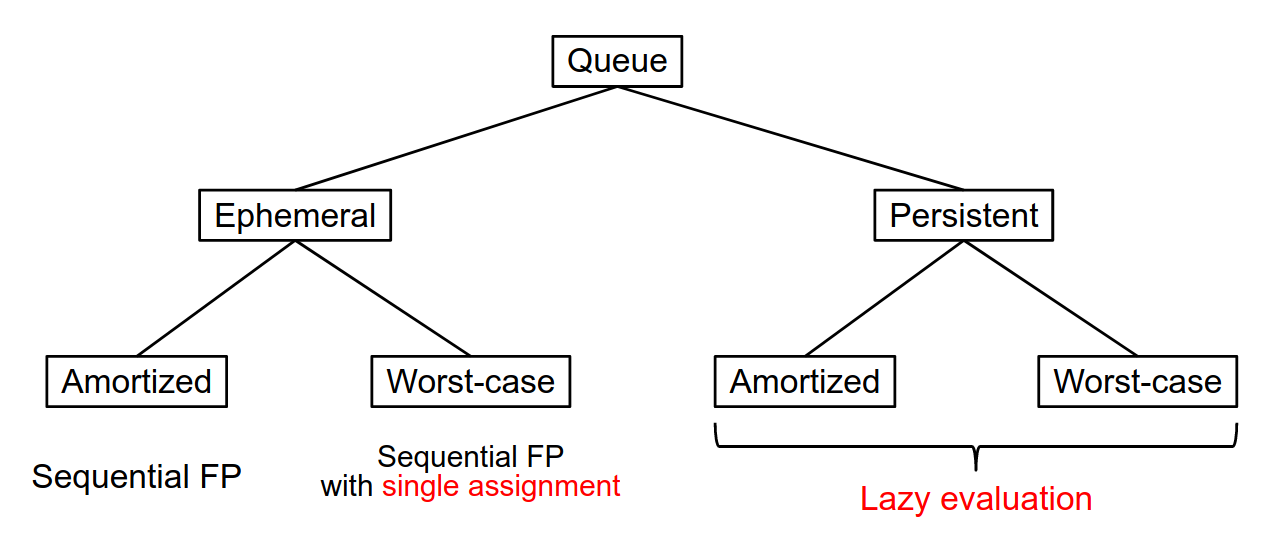
\includegraphics[scale=0.5]{img/Queue.png}
		
		\subsubsection{Amortzed Constant-tile Ephemeral Queue}
		Amortize O(1) car tous les insert se font en O(1) et le premier delete se fait en O(n) pour reverse la liste mais tant que elle est pas vide on reverse pas donc on peut delete encore n fois
		et éphemere car on change la liste a chauque fois et donc l'ancienne n'est plus utilisable apres
			\begin{lstlisting}[language=OZ]
%Queue represented as a tuple q(F R)  where element of the liste is {Append F {Reverse R}}
%Inserting is made on R and deleting on F
%If F is empty then {Reverse R} to F

fun{NewQueue} q(nil nil) end
fun{Check Q}
	case Q of q(nil R) then
		q({Reverse R} nil)
	else Q end
end

fun {Insert Q X}
	case Q of q(F R) then
		{Check q(F X|R)}
	end
end

fun {Delete Q X}
	case Q of q(F R) then F1 in
		F = X|F1
		{Check q(F1 R)}
	end
end

Q = {Insert {Insert {Insert {NewQueue} 1} 2 } 3}
Q1 = {Delete Q X}
			\end{lstlisting}
			
		\subsubsection{Worst-Case Constant Time Ephemeral Queue}
			Ici on crée des unbound variable au quelle on rajoute les élements ou retire
		exactement comme une difference liste
			
	
			\begin{lstlisting}[language=OZ]
%Queue represented as q(N S E) N the size and (S, E) a difference list, inserting by updating E et remove by updating S
fun{NewQueue} X in q(0 X X) end

fun {Insert Q X}
	case Q of q(N S E) then E1 in
		E = X|EI
		q(N+1 S E1)
	end
end

fun {Delete Q X}
	case Q of q(N S E) then S1 in
		S = X|S1
		q(N-1 S1 E)
	end
end
			\end{lstlisting}
			
		\subsubsection{Amortized Constant Time Persistent Queue}
			Le fait de la Lazy suspension du Reverse fait que c'est persistant. mais une fois Reverse appeler il est fait d'un cout car Monolithic
			
			\begin{lstlisting}[language=OZ]
fun{NewQueue} q(0 nil 0 nil) end

fun{Check Q}
	case Q of q(LenF F LenR R) then
		if LenF < LenR then
			q(LenF + LenR {Lappend F {fun lazy {$} {Reverse R} end}} 0 nil)
		else
			Q
		end
	end
end

fun {Insert Q X}
	Case Q of q(LenF F LenR R) then
		{Check LenF F LenR+1 X|R}
	end
end

fun {Delete Q X}
	case Q of q(LenF F LenR R) then F1 in
		F = X|F1
		{Check q(LenF-1 F1 LenR R)}
	end
end
			\end{lstlisting}
			
		\subsubsection{Worst-Case Constant-Time Persistent Queue}
			Le Append et reverse se font step par step et donc en O(1) donc pas de reverse direct en O(n)
			\begin{lstlisting}[language=OZ]
fun{NewQueue} q(0 nil 0 nil) end

fun lazy {LAppRev F R B}
	case pair(F R) of pair(X|F2 Y|R2) then
		X|{LAppRev F2 R2 T|B}
	[] pair(nil [Y]) then Y|B
	end
end

fun {Check Q}
	case Q of q(LenF F LenR R) then
		if lenF < LenR then
			q(LenF + LenR {LAppRev F R nil} 0 nil)
		else Q end
	end
end

fun {Insert Q X}
	case Q of q(LenF F LenR R) then
		{Check q(LenF F LenR+1 X|R)}
	end
end

fun {Delete Q X}
	case Q of q(LenF F LenR R) then F1 in
	F = X|F1
	{Check q(LenF-1 F1 LenR R)}
	end
end

			
			\end{lstlisting}
			
\section{Declarative Programming}
	\begin{center}
		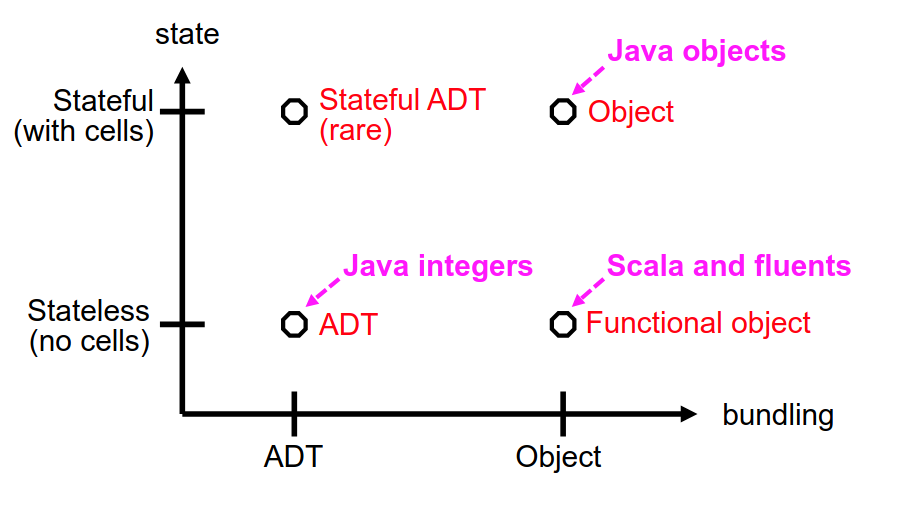
\includegraphics[scale=0.6]{img/ADT.png}
	\end{center}
	\subsection{Abstract DataType (ADT)}
		Set de valeur et operation\\Encapsulation avec des wrapper
		\begin{lstlisting}[language=OZ]
proc{NewWrapper Wrap UnWrap}
	Key = {NewName}
in
	fun{Wrap X} {Chunk.new w(Key:X)} end
	fun{UnWrap W} W.key end
end

Local Wrap UnWrap in
	{NewWrapper Wrap UnWrap}
	
	fun {NewStack} {Wrap nil} end
	fun {Push W X} {Wrap x|{UnWrap W}} end
	fun {Pop W X} S = {Unwrap W} in X = S.1 {Wrap S.2} end
end
		\end{lstlisting}
	\subsection{Object}
		représente valeurs et les opérations
		
		Pas déclaratif car state interne
		\begin{lstlisting}[language=OZ]
Fun {NewStack}
	C =  {NewCell nim}
	proc{Push X} C:= X|@C end
	proc{Pop X} S = @C in C:= S2 X = S.1 end
in
	proc{$ M}
		case M of push(x) then {Push X}
		[] pop(x) then {Pop X}
		end
	end
end
		\end{lstlisting}
	\subsection{Functional Object}
		Sans cellules, on utilise juste le static scope et le high order programming
			\begin{lstlisting}[language=OZ]
local
	fun {StackObject S}
		fun {Push X} {StackObject X|S} end
		fun {Pop X}
			case S of H|T then X=H {StackObject T} end
		end
	in
		stack(push:Push pop:Pop)
	end
in
	fun {NewStack} {StackObject nil} end
end
			\end{lstlisting}
			
	\subsection{Stateful ADT}
		\begin{lstlisting}[language=OZ]
		local Wrap UnWrap
			{NewWrapper Wrap UnWrap}
			
			fun {NewStack} {Wrap {NewCell nil}} end
			fun {Push S X} C ={Unwrap S} in C:=X|@C end
			fun {Pop S} C ={UnWrap S} in
				case @C of H|T then C:=T H end
			end
		in
			Stack = stack(new:NewStack push:Push pop:Pop)
		end
		\end{lstlisting}
		
\section{Messages Passing}
	\section{Server}
		Un server doit etre équitavle et le plus rapide possible, c'est pourquoi il est impossible de faire un server Non-déterministique car sinon les client serait dépendant de chaque un et cela ne serait plus dutout équitable si un client a le pouvoir sur d'autre
		\begin{lstlisting}[language=OZ]
fun {Server S}
	case S of H|T then
		{Handle H} %gerere le message H
		{Server T}
	end
end
		\end{lstlisting}	
	\section{FOLDL !!!}
		Le truc le plus important
		
		\begin{center}
			\includegraphics[scale=0.6]{img/fold.png}
		\end{center}
		\begin{lstlisting}[language=OZ]
fun {FoldL L F S}
	case L of H|T then
		{Fold T F {F S H}}
	[]nil then S
end
		\end{lstlisting}
	\section{StateFull port Object}
		\begin{lstlisting}[language=OZ]
fun {NewPortObject Init F}
	P 
	Out
in
	thread S in P={NewPort S} Out = {FoldL S F init}
		\end{lstlisting}
	\subsection{Active Object}
		\begin{lstlisting}[language=OZ]
fun {NewActive Class Init}
	Obj = {New Class Init}
	P
in
	thread S in
		P = {NewPort S}
		for M in S {Obj M} end
	end
	proc {$ M}{Send P M}
end
		\end{lstlisting}
		
	\subsection{Flavius Problem}
		\begin{lstlisting}[language=OZ]
class Victim
	attr ident alive step last succ pred
	
	meth init(I K L)
		alive := true
		step := K
		last := L
		Ident := I
	end
	
	meth setSucc(S) succ := S end
	meth setPred(P) pred := P end
	
	meth kill(X, S)
		if @alive then
			if S == 1 then
				@last = ident
			elseif (X mod @step == 0) then
				alive := false
				{@pred setSucc(@succ)}
				{@succ setPred(@pred)}
				{@succ kill(X+1 S-1)}
			else
				{@succ kill(X+1 S)}
			end
		end
	end
end

fun{Josephus N K}
	A = {NewArray 1 N null}
	Last
in 
	for I in 1..N do
		A.I := {New Active Victime init(I K Last)}
	end
	for I in 1..(N-1) do
		{A.I setSucc(A.I+1)}
	end
	{A.N setSucc(A.1)}
	
	for I in 2..(N) do
		{A.I setPred(A.I-1)}
	end
	{A.1 setPred(A.N)}
	{A.1 kill(K N)}
	
	Last
end
		\end{lstlisting}
	
\section{Multi-Agent Programming Erlang}
	\subsection{La base}
		\begin{lstlisting}[language=Erlang]
%Cree un processus
Pid = spawn(Fun).


%Traiter les messages recus dans la mailBox
receive
	Pattern1 -> Action1
	...
	PatternN -> ActionN
		\end{lstlisting}
		
\section{Shared State Concurency}
	\begin{center}
		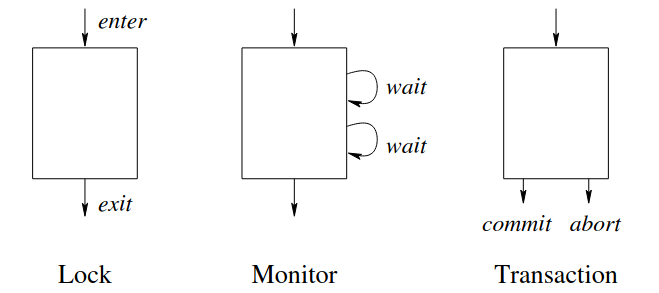
\includegraphics[scale=1]{img/Locks.png}
		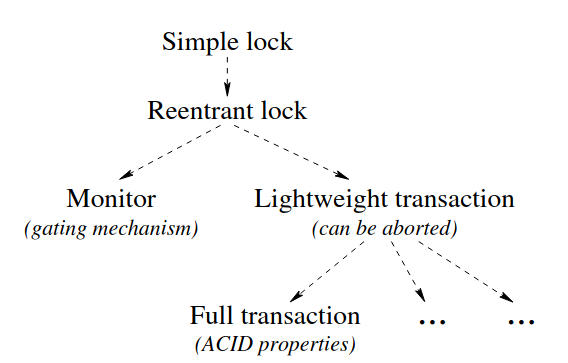
\includegraphics[scale=1]{img/Hierarchy.png}
	\end{center}
	
	\subsection{Lock}
		\subsubsection{Queue avec Lock}
			\begin{lstlisting}[language=OZ]
			
%% Avec le Lock
fun {NewQueue}
	X
	C = {NewCell q(0 nil nil)}
	L = {Lock}
	
	proc {Insert X} N F B2 in
		lock L then
			q(N F X|B) = @C
			C:= q(N+1 F B2)
		end
	end
	proc {Delete X} N F2 B in
		lock L then
			q(N X|F2 B) = @C
			C := q(N-1 F2 B)
		end
	end
in
	q(insert:Insert delete:Delete)
end

%Avec la fonction Exchange qui est atomique
fun {NewQueue}
	X
	C = {NewCell q(0 nil nil)}
	
	proc {Insert X} N F B2 M in
		{Exchange C q(N F X|B2) q(M F B2)} %Atomique aucun thread ne peut se glisser entre
		M = N+1
	end
	proc {Delete X} N F2 B M in
		{Exchange C q(N X|F2 B) q(M F2 B)}
		M = N+1
	end
in
	q(insert:Insert delete:Delete)
end
	
			\end{lstlisting}
		\subsubsection{Implémentation Lock}
			\begin{lstlisting}[language=OZ]
%% Pas reetrant
fun {SimpleToken}
	Token = {NewCell unit}
	proc{Lock P} Old New in
		{Exchange Token Old New}
		{Wait Old}
		{P}
		New = unit
	end
in
	lock(lock:Lock)
end		

%% Reetrant

fun {NewLock}
	Token = {NewCell unit}
	CurThr = {NewCell unit}
	
	proc{Lock P}
		if {Thread.this} == CurThr then
			{P}
		else Old New in
			{Exchange Token Old New}
			{Wait Old} %Entre section critique
			CurThr := {Thread.this}
			try {P} finally
				CurThr := unit
				New := unit % part section critique
			end
		end
	end
end
				
%% Queue avec Tuple Space
fun {NewQueue}
	X
	TS = {New TupleSpace init}
	proc {Insert X} N F B2 in
		{TS read(q q(N F X|B2))}
		{TS Write(q(N+1 F B2))}
	end
	
	proc{Delete X} N F2 B in
		{TS read(q q(N X|F2 B))}
		{TS write(q(N-1 F2 B))}
	end
in
	{TS write(q(0 X X))}
	queue(insert:Insert delete:Delete)
end
			\end{lstlisting}			
			
	\subsection{Monitor}
	\subsubsection{Buffer avec Monitor}
		\begin{lstlisting}[language=OZ]
class Buffer
	attr m buf first last n i
	meth init(N)
		m := {NewMonitor}
		buf := {NewArray 0 N-1 null}
		first := 0
		last := 0
		n := N
		i := 0
	end
	
	meth put(X)
		{@m.lock proc{$}
			if @i > @n then
				{@m.wait}
				{self.put(X)} % Toujours relancer car sinon Buggy
			else
				@buf.@last := X
				last := (@last + 1) mod @n
				i := @i + 1
				{@m.notifyAll}
			end		
		end}
	end
	
	meth get(X)
		{@m.lock proc{$} 
			if @i == 0 then
				{@m.wait}
				{self.get(X)} % Toujours relancer car sinon Buggy
			else
				X := @buf.@first
				first := (@first + 1) mod @n
				i:= @i - 1;
				{@m.notifyAll}
			end		
		end}
	end
end
		\end{lstlisting}
		\subsubsection{Implémentation}
		
		\begin{lstlisting}[language=OZ]
fun {NewGRLock}
	Token1 = {Newcell unit}
	Token2 = {Newcell unit}
	CurThr = {Newcell unit}
	
	fun{GetLock}
		if {Thread.this} == 0 then
			 Old New
		in
			{Exchange Token1 Old New}
			{Wait Old}
			Token2 = New
			CurThr = {Thread.this}
			true
		else
			false
		end
	end
	
	proc {ReleaseLock}
		CurThr := unit
		unit = @Token2 %Pass Token
	end
end

% Extended Queue
fun{NewQueue}
	X
	C = {NewCell q(0 X X)}
	L = {NewLock}
	
	proc {Insert X} N F B2 in
		lock L then
			q(N F X|B) = @C
			C:= q(N+1 F B2)
		end
	end
	proc {Delete X} N F2 B in
		lock L then
			q(N X|F2 B) = @C
			C := q(N-1 F2 B)
		end
	end
	
	fun {Size}
		lock L then @C.1 end
	end
	
	fun {DeleteAll}
		lock L then X S E in
			q(_ S E) = @C
			C := q(0 X X)
			E = nil
			S
		end
	end
	
	fun {DeleteNonBlock}
		lock l then
			if {Size} > 0 then [{Delete}]
			else nil end
		end
	end
in
	queue(insert:Insert delete:Delete size:Size deleteAll:DeleteAll deleteNonBlock:DeleteNonBlock)
end

%Monitor

fun {NewMonitor}
	Q = {NewQueue}
	L = {NewGRLock}
	
	proc {LockM P}
		if{L.get} then
			try {P} finally {L.release} end
		else {P} end
	end
	
	proc {WaitM} X in
		{Q.insert C}
		{L.release}
		{Wait X}
		if {L.get} then skip end
	end
	
	proc {NotifyM}
		U = {Q.deleteNonBlock} 
	in 
		case U of [X] then X=unit
		else skip end
	end
	
	proc{NotifyAllM}
		L={Q.deleteAll} 
	in
		for X in L do X=unit end
	end
	
end

		\end{lstlisting}
		        

















\end{document}